\section{大 O 符号}
当我们试图通过执行时间来表征算法的效率时,并且独立于任何特定程序或计算机,重要的是量化算法需要的操作或者步骤的数量。选择适当的基本计算单位是个复杂的问题,并且将取决于如何实现算法。对于先前的求和算法,一个比较好的基本计算单位是对执行语句进行计数。在 sumOfN 中,赋值语句的计数为 1 (theSum = 0) 加上 n 的值(我们执行 theSum=theSum+i 的次数)。我们通过函数 T 表示 T(n)=1 + n。参数 n 通常称为‘问题的规模’,我们称作 ‘T(n) 是解决问题大小为 n 所花费的时间,即 1+n 步长’。在上面的求和函数中,使用 n 来表示问题大小是有意义的。我们可以说,100,000 个整数和比 1000 个问题规模大。因此,所需时间也更长。我们的目标是表示出算法的执行时间是如何相对问题规模大小而改变的。
计算机科学家更喜欢将这种分析技术进一步扩展。事实证明,操作步骤数量不如确定 T(n) 最主要的部分来的重要。换句话说,当问题规模变大时,T(n) 函数某些部分的分量会超过其他部分。函数的数量级表示了随着 n 的值增加而增加最快的那些部分。数量级通常称为大O符号,写为 O(f(n))。它表示对计算中的实际步数的近似。函数 f(n) 提供了 T(n) 最主要部分的表示方法。
在上述示例中,T(n)=1+n。当 n 变大时,常数 1 对于最终结果变得越来越不重要。如果我们找的是 T(n) 的近似值,我们可以删除 1, 运行时间是 O(n)。要注意,1 对于 T(n) 肯定是重要的。但是当 n 变大时,如果没有它,我们的近似也是准确的。
另外一个示例,假设对于一些算法,确定的步数是 $T(n)=5n^2 +27n+1005$。当 n 很小时, 例如 1 或 2 ,常数 1005 似乎是函数的主要部分。然而,随着 n 变大,$n^2$ 这项变得越来越重要。事实上,当 n 真的很大时,其他两项在它们确定最终结果中所起的作用变得不重要。当 n 变大时,为了近似 T(n),我们可以忽略其他项,只关注 $5n^2$ 。系数 5 也变得不重要。我们说,T(n) 具有的数量级为 $f(n)=n^2$。 或者 $O( n^2 )$ 。
虽然我们没有在求和示例中看到这一点,但有时算法的性能取决于数据的确切值,而不是问题规模的大小。对于这种类型的算法,我们需要根据最佳情况,最坏情况或平均情况来表征它们的性能。最坏情况是指算法性能特别差的特定数据集。而相同的算法不同数据集可能具有非常好的性能。大多数情况下,算法执行效率处在两个极端之间(平均情况)。对于计算机科学家而言,重要的是了解这些区别,使它们不被某一个特定的情况误导。
当你学习算法时,一些常见的数量级函数将会反复出现。见 Table 1。为了确定这些函数中哪个是最主要的部分,我们需要看到当 n 变大的时候它们如何相互比较。

\begin{table}[htbp]
\centering
\begin{tabular}{|c|l|}\hline
$O(1)$ & Constant \\
$O(\log n)$ & Logarithmic\\
$O(n)$ & Linear\\
$O(n \log n)$ & Log Linear\\
$O(n^2)$ & Quadratic\\
$O(n^3)$ & Cubic\\
$O(2^n)$ & Exponetial\\\hline
\end{tabular}
\end{table}

Figure 1 表示了 Table 1 中的函数图。注意,当 n 很小时,函数彼此间不能很好的定义。很难判断哪个是主导的。随着 n 的增长,就有一个很明确的关系,很容易看出它们之间的大小关系。


\begin{figure}[htbp]
        \centering
        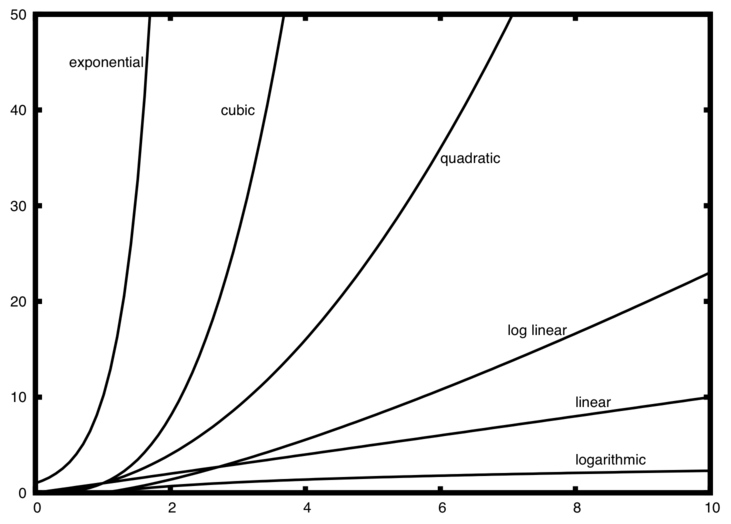
\includegraphics[width=4in]{images/newplot.png}
\end{figure}

最后一个例子,假设我们有 Listing2 的代码段。虽然这个程序没有做任何事,但是对我们获取实际的代码和性能分析是有益的。
\lstinputlisting{code/ex1.py}

分配操作数分为四个项的总和。第一个项是常数 3, 表示片段开始的三个赋值语句。第二项是 $3n^2$, 因为由于嵌套迭代,有三个语句执行 $n^2$ 次。第三项是 2n, 两个语句迭代 n 次。最后,第四项是常数 1,表示最终赋值语句。最后得出 $T(n)=3+3n^2 +2n+1=3n^2 + 2n+4$,通过查看指数,我们可以看到 $n^2$ 项是显性的,因此这个代码段是 $O(n^ 2 )$。当 n 增大时,所有其他项以及主项上的系数都可以忽略。
\begin{figure}[htbp]
        \centering
        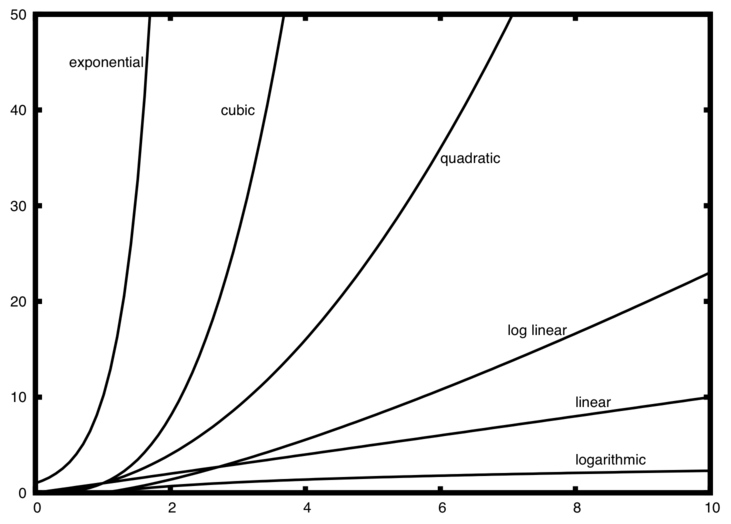
\includegraphics[width=4in]{images/newplot.png}
\end{figure}
Figure 2 展示了一些常用的 大O 函数,跟上面讨论的 T(n) 函数比较,一开始的时候,T(n) 大于三次函数,后来随着 n 的增长,三次函数超过了 T(n)。T(n) 随着二次函数继续增长。

